%! TEX root = main.tex
The second part of our benchmarking with PINNs focuses on the ability to simulate sensitive dynamical systems of flow problems.
Our benchmark target is the 2D cylinder flow of $Re=200$, which exhibits vortex shedding.
However, before we conduct the benchmark on the $Re=200$ cylinder flow, we would like to test a steady cylinder flow problem with our unsteady PINN implementation for solver validation.
The selected case is an $Re=40$ cylinder flow, which reaches a steady state eventually.
The results were validated with experimental data and verified against PetIBM results.

The computational domain of the $Re=40$ cylinder flow is $[-10, 30]\times[-10, 10]$, and the simulation time range is $t=0$ to $t=20$.
A cylinder with a radius of $0.5$ sits at the coordinate $(0, 0)$.
Nondimensional density is $1$ and kinematic viscosity is $0.025$ so that the Reynolds number is $40$.
The IC is $u=1$ and $v=0$.
The BCs are $u=1$ and $v=0$ on $x=-10$, $y=-10$, and $y=10$.
The BC at the outlet $x=30$ is a 1D convective condition:
\begin{equation}\label{eq:convec-bc}
    \left\{
    \begin{aligned}
        &\pdiff{u}{t} + c\pdiff{u}{\vec{n}} = 0 \\
        &\pdiff{v}{t} + c\pdiff{v}{\vec{n}} = 0 \\
    \end{aligned}
    \right.
\end{equation}
where $\vec{n}$ is the normal vector of the boundary pointing outward from the domain, and $c$ is the convection speed.
In this work, we used $c=1$.

The network used is $(N_l, N_n)=(6, 512)$.
Two PINN implementations were used: a steady solver and an unsteady one.
Two different $N_{bs}$ were used as well to confirm the effect of batch sizes we observed in the previous section: $N_{bs}=6400$ and $N_{bs}=25,600$.
And we tested two different cyclical learning rate configurations:
\begin{enumerate}[nolistsep]
    \item Large cycle: $(\eta_{low}, \eta_{high}, N_c, \gamma)=(1e-6, 1e-2, 5000, 0.99998)$
    \item Small cycle: $(\eta_{low}, \eta_{high}, N_c, \gamma)=(1e-6, 1e-3, 2000, 0.999972)$
\end{enumerate}
Figure \ref{fig:cylinder-2d-re40-lr-hist} shows the comparison of the two scheduling.
\begin{figure}[hbt!]
    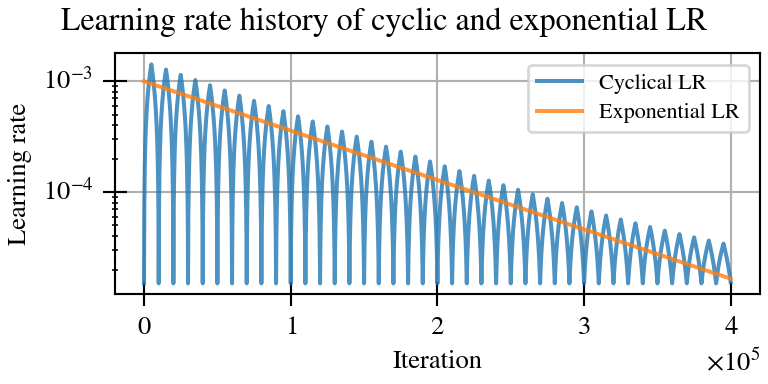
\includegraphics[width=0.9\linewidth]{cylinder-2d-re40/learning-rate-hist}
    \caption[
        PINNs, 2D Cylinder, $Re=40$: cyclical learning rate configurations%
    ]{%
        PINNs, 2D Cylinder, $Re=40$: cyclical learning rate configurations%
    }%
    \label{fig:cylinder-2d-re40-lr-hist}
\end{figure}
A total of 6 cases were run in this benchmark.
(The $N_{bs}=25,600$ was not applied to small cycle scheduling.)

For unsteady cases with $N_{bs}=6,400$, $6,400\times 10,000$ points were sampled from the computational spatial-temporal domain for PDE losses, meaning each batch was repeated every $10,000$ iterations.
Except for the cylinder surface, $640\times 10,000$ points were sampled on each boundary and $t\in[0, 20]$.
On the cylinder surface, $256\times 10,000$ points were sampled and also with $t\in[0, 20]$.
To evaluate IC losses, $6,400\times 10,000$ points were sampled from the spatial domain with their temporal coordinates being limited to $t=0$.
The steady cases with $N_{bs}=6,400$ follows a similar setting, except the PDE evaluation points were sampled completely from spatial domain, as there was no temporal coordinates.
And steady cases did not need to evaluate IC losses.

For cases with $N_{bs}=25,600$, the PDE evaluation points follow the same logic described above.
We used $2,560\times 10,000$ points on the boundaries of $y=\pm 10$ and $1,280\times 10,000$ points on the boundaries of $x=-10$ and $x=30$.
The cylinder surface had $512\times 10,000$ points.

Each case ran for 400,000 iterations during optimization with the Adam optimizer.
The hardware used was 1 NVIDIA A100 GPU for all cases.

A PetIBM simulation was done as a baseline.
The simulation ran with an NVIDIA K40 GPU with 6 cores of Intel i7-5930K.
Note that K40 GPU is 5 generations behind the A100 GPU in terms of the technology specification.
The PetIBM simulation resolved the flow on a $562 \times 447$ stretched Cartesian grid with the same computational spatial-temporal domain.
PetIBM used double-precision floats, while PINNs used single precision floats.
The tolerance for all linear solvers in PetIBM was $1e-14$.
% vim:ft=tex